In many decision-making applications---ranging from logistics and finance to
energy systems and scheduling---problems can be naturally modeled as
mixed-integer optimization problems (MIPs). These problems combine continuous
and integer variables to represent decisions under various logical,
structural, or operational constraints.

In \textsf{idol}, we adopt a general and flexible framework for expressing
such problems. A MIP is assumed to be of the following form:
\begin{subequations}
    \begin{align}
        \min_x \quad & c^\top x + x^\top D x + c_0 \\
        \text{s.t.} \quad 
        & a_{i\cdot}^\top x + x^\top Q^i x \le b_i, \quad \text{for all } i=1,\dotsc,m, \\
        & \ell_j \le x_j \le u_j, \quad \text{for all } j = 1,\dotsc,n, \\
        & x_j\in \mathbb{Z}, \quad \text{for all } j\in J \subseteq\{1,\dotsc,n\}. \label{eq:mip:integer-requirements}
    \end{align}
    \label{eq:mip}
\end{subequations}
Here, $x$ is the decision variable vector, and the input data are as follows:
Vector $c \in \mathbb{Q}^n$, matrix $D\in\mathbb{Q}^{n\times n}$ and the
constant $c_0 \in \mathbb{Q}$ define the linear, the quadratic and the
constant parts of the objective function, respectively; For each constraint
with index $i\in\{1,\dotsc,m\}$, vector $a_{i\cdot}$, matrix $Q^i \in
\mathbb{Q}^{n \times n}$ and constant $b_i$ encode the linear part, the
quadratic part, and the right-hand side of the constraint respectively;
Vectors $\ell \in \mathbb{Q}^n \cup \{-\infty\}$ and $u \in \mathbb{Q}^n \cup
\{\infty\}$ are used to define lower and upper bounds on each variables; Finally, the
set $J \subseteq \{1, \dotsc, n\}$ specifies which variables are required to
be integer.

As is customary, variables are classified depending on their type---which can
be continuous, integer or binary---and bounds. This is presented in
Table~\ref{tab:var-types}. As to constraints, they are said to be linear when
$Q^i = 0$, and quadratic otherwise. Likewise, the objective function is
quadratic when $D \ne 0$. 

\begin{table}
    \caption{Terminology for variables in a MIP.}
    \label{tab:var-types}
    \begin{tabular}{ll}
        \toprule
        A variable $x_j$ is said ... & if it satisfies ... \\\midrule
        integer & $j\in J$ \\
        binary & $j\in J$ and $0 \le \ell \le u \le 1$ \\
        continuous & $j\notin J$ \\\midrule
        free & $l=-\infty$ and $u = \infty$ \\
        non-negative & $\ell \ge 0$ \\
        non-positive & $u \le 0$ \\
        bounded &  $-\infty < \ell \le u < \infty$ \\
        fixed &  $\ell = u$ \\\bottomrule
    \end{tabular}
\end{table}

A particularly important subclass of MIPs arises when both the constraints and
the objective function are linear (i.e., $Q^i = 0$ for all $i$ and $D = 0$).
In this case, the problem is known as a mixed-integer linear problem (MILP).

For many practical purposes, it is helpful to consider the continuous
relaxation of a MIP. This is obtained by removing the integrality
constraints~\eqref{eq:mip:integer-requirements}, allowing all variables to
take real values. This relaxation is easier to solve and often provides useful
bounds or insights about the original problem.

\subsection*{Disclaimer}
You do not need to read every section in detail before solving your first
problem. Most users can start with the example in
Section~\ref{sec:milp-example}, which demonstrates how to define a basic MILP
using \textsf{idol}. Later sections dive deeper into the modeling framework,
including variables, constraints, and the environment that manages them.
%
Note that solving a model (i.e., computing an optimal point) is not covered in
this chapter. This is the focus of the next chapter, where you will learn
about how to use an~\textsf{Optimizer} and an~\textsf{OptimizerFactory}.

\section{Example: a toy mixed-integer linear problem}
\label{sec:milp-example}

To illustrate the modeling capabilities of \textsf{idol}, we begin with a
small example which is a mixed-integer linear program (MILP). 
%
The mathematical model reads:
\begin{subequations}
    \label{eq:milp-example}
    \begin{align}
        \min_x \quad & -x - 2y \\
        \text{s.t.} & -x + y \le 1, \\
        & 2x + 3y \le 12, \\
        & 3x + 2y \le 12, \\
        & x,y\in\mathbb{Z}_{\ge 0}.
    \end{align}
\end{subequations}
This is a minimization problem which involves two integer variables, $x$ and
$y$, both constrained to be non-negative. The feasible region is defined by
three linear inequalities. Figure~\ref{fig:milp-example} shows this region
(shaded in blue), the integer-feasible points, and the direction of the
objective function (represented by the vector $-c$).
%
The continuous relaxation of this problem---where $x$ and $y$ are allowed to
take real values---has a unique solution at $(x^*, y^*) = (2.4, 2.4)$, with an
objective value of $-7.2$. The original integer-constrained problem also
admits a unique solution at $(x^*, y^*) = (2, 2)$, with objective value $-5$.

\newcommand{\drawPoint}[2]{\filldraw[orange] (#1,#2) circle (1.5pt) node[anchor=north west] {};}

\begin{figure}
    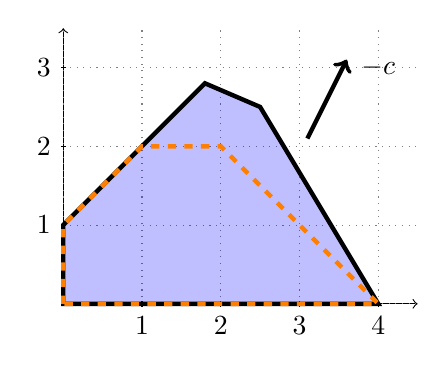
\begin{tikzpicture}
        \draw[<->] (0,3.5) |- (4.5,0);

        \foreach \x in {0,...,4}
            \draw[gray, dotted] (\x,0) -- (\x,3.5);
        \foreach \y in {0,...,3}
            \draw[gray, dotted] (0,\y) -- (4.5,\y);

        \draw[fill=blue, ultra thick, fill opacity=.25] (0,0) -- (0,1) -- (1.8,2.8) -- (2.5,2.5) -- (4,0) -- cycle;

        % Draw ticks on x-axis
        \foreach \x in {1,2,3,4}
            \draw (\x cm,1pt) -- (\x cm,-1pt) node[anchor=north] {$\x$};
        
        % Draw ticks on y-axis
        \foreach \y in {1,2,3}
            \draw (1pt,\y cm) -- (-1pt,\y cm) node[anchor=east] {$\y$};

        \draw[->,ultra thick,black] (3.1,2.1) -- (3.6,3.1);
        \draw (4,3) node {$-c$};
        
        \draw[ultra thick, orange, dashed] (0,0) -- (0,1) -- (1,2) -- (2,2) -- (4,0) -- cycle;

        \drawPoint{0}{0}
        \drawPoint{1}{0}
        \drawPoint{2}{0}
        \drawPoint{3}{0}
        \drawPoint{4}{0}
        
        \drawPoint{0}{1}
        \drawPoint{1}{1}
        \drawPoint{2}{1}
        \drawPoint{3}{1}

        \drawPoint{1}{2}
        \drawPoint{2}{2}

    \end{tikzpicture}
    \caption{Feasible region (shaded in blue) for
    Problem~\eqref{eq:milp-example}, with integer-feasible points highlighted
    and objective direction shown.}
    \label{fig:milp-example}
\end{figure}

Modeling Problem~\eqref{eq:milp-example} in~\textsf{idol} is straightforward.
In particular, if you are familiar with other optimization packages like
\textsf{JuMP} in~\textsf{Julia} or the \textsf{Gurobi} \textsf{C++} API,
the following code snippet should be easy to understand.
%
\begin{lstlisting}
#include <iostream>
#include "idol/modeling.h"

using namespace idol;

int main(int t_argc, const char** t_argv) {

    Env env; @\label{code:create-env}@

    // Create a new model.
    Model model(env); @\label{code:create-model}@

    // Create decision variables x and y.
    const auto x = model.add_var(0, Inf, Integer, -1, "x"); @\label{code:create-variable-x}@
    const auto y = model.add_var(0, Inf, Integer, -2, "y"); @\label{code:create-variable-y}@

    // Create constraints.
    const auto c1 = model.add_ctr(-x + y <= 1); @\label{code:create-constraint-c1}@
    const auto c2 = model.add_ctr(2 * x + 3 * y <= 12);
    const auto c3 = model.add_ctr(3 * x + 2 * y <= 12); @\label{code:create-constraint-c3}@

    return 0;
}

\end{lstlisting}

Let's walk through this code. In Line~\ref{code:create-env}, we create a new
optimization environment that will store all our optimization objects such as
variables or constraints. Destroying an environment automatically destroys all
objects which were created with this environment. Then, in
Line~\ref{code:create-model}, we create an optimization model. By default, all
models are for minimization problems. Decision variables are created in
Lines~\ref{code:create-variable-x} and~\ref{code:create-variable-y}. There, we
set the lower bound to 0 and an infinite upper bound using the defined
constant $\textsf{idol::Inf}$. Both variables are defined as~\textsf{Integer}.
Note that other types are possible, e.g., \textsf{Continuous} and
\textsf{Binary}. The objective coefficients are also set in these lines by the
fourth argument. The last argument corresponds to the internal name of that
variable and is mainly useful for debugging. Finally,
Lines~\ref{code:create-constraint-c1}--\ref{code:create-constraint-c3} add
constraints to the model to define the feasible region of the problem.

Note that, as such, we are only modeling Problem~\eqref{eq:milp-example} here
but we are not performing any optimization task so far. This is the subject of
the next chapter. For the sake of completeness, however, here is how one uses
the commercial solver~\textsf{Gurobi} to compute a solution
of this problem.
%
\begin{lstlisting}
    model.use(Gurobi());
    model.optimize();

    std::cout << "Status = " << model.get_status() << std::endl;
    std::cout << "x = " << model.get_var_primal(x) << std::endl;
    std::cout << "y = " << model.get_var_primal(y) << std::endl;
\end{lstlisting}

This prints the solution status (here, \textsf{Optimal}) and the values of the
decision variables in the solution (here, $(x^*,y^*) = (2,2)$). 

\section{The environment}

Any optimization object---such as variables, constraints and models---are
managed through a central entity called an ``optimization environment''.
This environment, represented by the \textsf{Env} class, acts as a container 
and controller for all optimization-related objects created within its scope.

The environment has two key responsabilities:
\begin{enumerate}
    \item \textbf{Lifecycle management.} When an environment is destroyed, all
    objects created within it are automatically deleted. This eliminates the
    need for manual memory management. Also, once an object is no longer
    referenced, it is safely cleaned up by the environment, i.e., you do not
    need to manually delete objects.
    \item \textbf{Version tracking.} During the execution of an optimization
    program, objects like variables and constraints may appear in different
    models with model-specific changes. These different versions of a single
    object are all stored and managed in the environment.  
\end{enumerate}

Typically, a single environment should suffice for most applications. While
\textsf{idol} technically allows the creation of multiple environments, this
is strongly discouraged. Objects created in one environment must not be mixed
with those from another. For example, attempting to add a variable from one
environment to a model belonging to a different environment will lead to
undefined behavior, often resulting in segmentation faults or program crashes.

Creating an environment is straightforward:
%
\begin{lstlisting}
    Env env; // Creates a new optimization environment.
\end{lstlisting}

Once initialized, you can begin creating models, variables, and constraints
using this environment. All such objects will be associated with \textsf{env}
and managed accordingly throughout their lifetime.

\section{Models}

Mathematical optimization problems are modeled using the \textsf{Model} class.
A model is a set of variables and constraints with an objective function. It
can be created by calling the constructor of the \textsf{Model} class by
passing an environment as the first argument.

\begin{lstlisting}
    Env env;
    Model model(env); // Creates an empty model.
\end{lstlisting}

Here, we first create a new optimization environment, then create an
optimization model. Note that the newly created model does not contain any
variable nor constraints. By default, all models are for minimization
problems. Unfortunately, idol offers limited support for maximization problem.
However, it is well knwon that this is not a real restriction since $\max f(x)
= - \min -f(x)$. 

Another way to create a model is by importing it from an \textsf{.mps} or
an~\textsf{.lp} file. To do this, you will need to rely on an external solver.
In what follows, we use~\textsf{GLPK}, which is an open-source solver which
can be easily installed on your computer.

\begin{lstlisting}
    Env env;
    auto model = GLPK::read_from_file("/path/to/some/file.mps");
\end{lstlisting}

The choice to rely on external solver is justified by the fact that, first of
all, \textsf{idol} will most of the time be used in combination with such a
solver to effectively solve optimization problems. Second, it is also safer to
rely on existing codes with years of experience to import your model without
mistake or ambiguity.

Now that we have a model imported, we can safely iterate over its variables
and constraints. This can be done as follows. 

\begin{lstlisting}
    for (const auto& var : model.vars()) {
        std::cout << var.name() << std::endl;
    }
\end{lstlisting}
Here, we use the \textsf{Model::vars()} method to get access to the variables
of the model and write down their names. Note that you can also use the
\textsf{operator<<(std::ostream\&, const Model\&)} function to print the model
to the console. This can be useful for debugging. 

Once we have iterated over the variables, we may want to iterate over
constraints as well. To do so, we can use: the \textsf{Model::ctrs()} method
for linear constraints,  the \textsf{Model::qctrs()} method for quadratic
constraints and the \textsf{Model::sosctrs()} method for SOS-type constraints.
The next code snippet shows how to get the number of variables and
constraints.

\begin{lstlisting}
    std::cout << "Number of variables: " 
              << model.vars().size() << std::endl;

    std::cout << "Number of linear constraints: "
              << model.ctrs().size() << std::endl;

    std::cout << "Number of quadratic constraints: "
              << model.qctrs().size() << std::endl;

    std::cout << "Number of sos-type constraints: "
              << model.sosctrs().size() << std::endl;
\end{lstlisting}

To get model-specific information about a variable, a constraint or the
objective function, we can use methods like \textsf{Model::get\_X\_Y(const
X\&)} where \textsf{X} is an object name---like \textsf{var}, \textsf{ctr},
\textsf{qctr}, \textsf{sosctr} or \textsf{obj}---and \textsf{Y} is the data
name you which to gain access---like \textsf{lb}, \textsf{type} or
\textsf{column}. For instance, the following code counts the number of binary
variables in the model.

\begin{lstlisting}
    unsigned int n_binary_vars = 0;

    // Iterate over all variables in the model.
    for (const auto& var : model.vars()) {

        // Get the variable type in this model.
        const auto type = model.get_var_type(var);

        // Check type is binary.
        if (type == Binary) {
            ++n_binary_vars;
        }

    }
\end{lstlisting}

Complete details on what information you can retrieve through a model will be
detailed in the following sections. 

In most practical cases, you will want to avoid copying a model but, rather,
pass on a reference to some auxiliary function. For that reason, the copy
constructor of the \textsf{Model} class is declared as \textsf{private}. If
copying a model is really what you intend to do, you should use the
\textsf{Model::copy()} method and the move constructor. Here is an example. 

\begin{lstlisting}
    const auto model = Gurobi::read_from_file("problem.lp");
    auto model2 = model.copy();
\end{lstlisting}
Here, \textsf{model2} is now an independent copy of the original model and can
be modified without altering its source model. Similarly, if you want to write
a function that returns a model, you will have to be explicit about it to
avoid unncessary copies. See the following code.

\begin{lstlisting}
    Model read_model_from_file() {
        
        // Read the model from the file.
        auto model = Gurobi::read_from_file("problem.lp");

        // Use std::move to avoid unnecessary copies.
        // If a copy is intended, use Model::copy().
        return std::move(model); 
    }
\end{lstlisting}

Moving the model instead of copying it avoids the overhead of duplicating
large optimization problems.

\section{Variables}

Variables are the decision-making elements of an optimization problem. These
are the quantities that we aim to determine in order to optimize an objective
function, subject to a set of constraints. In \textsf{idol}, they are
represented by the \textsf{Var} class. 

\subsection{Creating variables}

Creating variables can be done in mainly two ways. The first one is through
the \textsf{Var} constructor and the \textsf{Model::add()} method, while the
second uses the \textsf{Model::add\_var(...)} methods. We start with the fist
method which uses the \textsf{Var} constructor. This method is less direct,
but more informative on how optimization objects are managed in~\textsf{idol}.
We focus on the following constructor:
\begin{center}
    \textsf{Var(Env\&, double, double, VarType, double, std::string)}.
\end{center}
This constructor takes six arguments. The first is the optimization
environment which will store the variable's versions. The two subsequent are
the lower and upper bound---possibly infinite using \textsf{idol::Inf}.
Then, the type of the variable is expected---such as
\textsf{idol::Continuous}, \textsf{idol::Integer} or \textsf{idol::Binary}.
The linear coefficient of the variable in the objective function is the fifth
argument. Finally, the last argument is the given name of the variable. For
instance, the following code creates a new variable in the environment.

\begin{lstlisting}
    Var x(env, 0, Inf, Continuous, 2, "x");
\end{lstlisting}
This variable is a continuous non-negative variable with an objective
coefficient of 2. It is called ``\textsf{x}''. One important thing is that
this variable does not belong to any model yet. Instead, what we have created
is called the ``default version'' of the variable. This means that, by
default, if this variable is added to a model, it will have the corresponding
attributes in that model. For instance, here is a code that creates and add
this variable to a model.

\begin{lstlisting}
    // Create a variable in the environment.
    Var x(env, 0, Inf, Continuous, 2, "x");

    // Add the variable to a model 
    model.add(x);
\end{lstlisting}

By default, the variable ``\textsf{x}'' is added to the model as a continuous
non-negative variable with an objective coefficient of 2. Note that other
constructors are also available in the \textsf{Var} class. For instance, it is
also possible to provide a column associated to the variable so that it is
automatically added to the LP matrix. Columns are built using the
\textsf{LinExpr<Ctr>} class and can be built in a very natural way. For more
details, please refer to Section~\ref{sec:expressions} on expressions in
\textsf{idol}. We simply give one example. 

\begin{lstlisting}
    // This function is assumed to return a vector of constraints.
    const std::vector<Ctr> ctrs = get_vector_of_ctrs(); 

    // Create the column associated to x.
    LinExpr<Ctr> column = -1 * c[0] + 2 * c[1] + 3 * c[2];

    // Create a variable in the environment.
    Var x(env, 0, Inf, Integer, -1, std::move(column), "x");

    // Add the variable to a model.
    model.add(x);
\end{lstlisting}

Finally, note that it is possible to avoid adding the default version to a
model by overriding it as follows. 

\begin{lstlisting}
    // Add the variable to a model, overriding the default version. 
    model.add(x, TempVar(0, Inf, Continuous, 2, LinExpr<Var>()));
\end{lstlisting}

Here, we notice the use of the \textsf{TempVar} class. This class is a
lightweight class used to represent a variable that has yet not been created
inside an environment. As such, it contains all attributes of the variable to
be created but it cannot be used other than for storing these attributes and
create an actual variable.

The second approach for creating variables is more straightforward. However,
it internally is exactly the same as what we have seen so far. This can be
reached using the \textsf{Model::add\_var} methods from the \textsf{Model}
class. The following code snippet should be easy to understand.

\begin{lstlisting}
    const auto x = model.add_var(0, Inf, Continuous, 2, "x");
\end{lstlisting}
Note that we do not need to pass the environment since the environment of the
model is automatically used. Also, two operations are performed in a single
call here: first, a default version is created for the variable, then the
variable is added to the model. Similarly, it is also possible to add a
variable with a specific column in the LP matrix. 

Sometimes, you will find it more convenient to create several variables at
once. This can be done by calling the \textsf{Var::make\_vector} function, or
the \textsf{Model::add\_vars} method. These functions require one extra
parameter specifying the dimension of the new variable. For instance, here is
how to create a set of variables with a $2\times 3$ index.

\begin{lstlisting}
    // Create a 2x3 "vector" of variables.
    const auto x = Var::make_vector(env, Dim<2>(2, 3), 0, Inf, Continuous, "x");

    // Add all variables
    model.add_vector<Var, 2>(x);

    // Print the first variable's name.
    std::cout << "x_0_0 = " << x[0][0].name() << std::endl;
\end{lstlisting}

Notice that we used the \textsf{Dim} class to specify the dimensions. The
\textsf{Dim} class is a template class that takes an integer as parameter.
This integer specifies the number of indices for the new variable. In this
case, we use 2 to specify that we want to create a two-dimensional index.
Then, we give the size of each dimension by passing the appropriate arguments
to the constructor of the \textsf{Dim} class, i.e., 2 and 3. 

Naturally, it is also possible to achieve this goal through methods of the
\textsf{Model} class. The following snippet gives an example.

\begin{lstlisting}
    const auto x = model.add_vars(Dim<2>(2,3), 0, Inf, Continuous, "x");
\end{lstlisting}

\subsection{Removing variables}

Once a variable has been added to a model, it can also be removed from it. We
use the \textsf{Model::remove(const Var\&)} method for this. Calling this
method will remove the variable from the model and update all linear and
quadratic constraints where this variable appeared. Trying to remove a
variable which does not belong to a model will result in an exception being
thrown. However, it is possible to check whether a model has a given variable
using the \textsf{Model::has(conv Var\&)} method. This method returns true if
and only if the variable is part of the model. Also, note that it is not
possible to remove a variable which is involved in an SOS-type constraint.
This is not limiting since SOS-type constraints can be removed and added
again.

\subsection{Accessing variables}

Variables have two immutable attributes: a name, which is the given name at
creation time of the variable and an id, which is unique in the environment.
Other attributes are tied to a specific model and can be accessed through the
model's methods \textsf{Model::get\_var\_Y} where \textsf{Y} is the name of
that attribute. Next is list of methods which can be used to retrieve
information about variables in a model.
%
\begin{description}
    \item[\textsf{double Model::get\_var\_lb(const Var\&)}]\hphantom{.}\\
    Returns the lower bound of the variable given as parameter. \\
    May return any value between \textsf{-idol::Inf} and \textsf{idol::Inf}.
    \item[\textsf{double Model::get\_var\_ub(const Var\&)}]\hphantom{.}\\
    Returns the upper bound of the variable given as parameter. \\ 
    May return any value between \textsf{-idol::Inf} and \textsf{idol::Inf}.
    \item[\textsf{double Model::get\_var\_obj(const Var\&)}]\hphantom{.}\\
    Returns the objective coefficient in the linear part of the objective
    function.
    \item[\textsf{VarType Model::get\_var\_type(const Var\&)}]\hphantom{.}\\
    Returns the type of the variable which can be \textsf{Continuous},
    \textsf{Integer} or \textsf{Binary}.
    \item[\textsf{LinExpr<Ctr> Model::get\_var\_column(const Var\&)}]\hphantom{.}\\
    Returns the associated column in the LP matrix.
    \item[\textsf{unsigned int Model::get\_var\_index(const Var\&)}]\hphantom{.}\\
    Returns the index of the variable. \\ 
    Note that this index may change if variables are removed.
\end{description}

We now give an example which prints out all free variables. 

\begin{lstlisting}
    for (const auto& var : model.vars()) {

        const double lb = model.get_var_lb(var);
        const double ub = model.get_var_ub(var);

        if (is_neg_inf(lb) && is_pos_inf(ub)) {
            std::cout << var.name() << " is free." << std::endl;
        }

    }
\end{lstlisting}

One final note regarding indices. Though they may change over time, e.g., if
variables are removed from a model, it can still be used to access variables
by using the \textsf{Model::get\_var\_by\_index} method. The following code
snippet shows an alternative way to iterate over variables in a model. 

\begin{lstlisting}
    for (unsigned int i = 0, n = model.vars().size(); i < n; ++i) {
        
        // Get the variable by index
        const auto& var = model.get_var_by_index(i);
        
        // Print out its name
        std::cout << var.name() << std::endl;

    }
\end{lstlisting}

\subsection{Modifying variables}

Some of the attributes of a variable may be directly changed through the
model's methods \textsf{Model::set\_var\_Y}. Here again, \textsf{Y} is the
name of the attribute you wish to modify. Here is a list of methods to be used
for modifying attributes of a variable in a model.
%
\begin{description}
    \item[\textsf{void Model::set\_var\_lb(const Var\&, double)}]\hphantom{.}\\ 
    Sets the lower bound of a variable. \\
    The new lower bound can be \textsf{-idol::Inf}, \textsf{idol::Inf} or any
    double in between. 
    \item[\textsf{void Model::set\_var\_ub(const Var\&, double)}]\hphantom{.}\\ 
    Sets the lower bound of a variable. \\
    The new lower bound can be \textsf{-idol::Inf}, \textsf{idol::Inf} or any
    double in between. 
    \item[\textsf{void Model::set\_var\_obj(const Var\&, double)}]\hphantom{.}\\ 
    Sets the linear coefficient in the objective function. 
    \item[\textsf{void Model::set\_var\_type(const Var\&, VarType)}]\hphantom{.}\\ 
    Sets the type of a variable. \\
    Changing the type of variable does not affect its bounds. 
    \item[\textsf{void Model::set\_var\_column(const Var\&, const LinExpr<Ctr>\&)}]\hphantom{.}\\ 
    Sets the column of a variable in the LP matrix. 
\end{description}

We end with an example which copies a model and creates its continuous
relaxation.

\begin{lstlisting}
    // Copy the model.
    auto continuous_relaxation = model.copy();

    // Build the continuous relaxation. 
    for (const auto& var : model.vars()) {
        continuous_relaxation.set_var_type(var, Continuous);
    }
\end{lstlisting}

\section{Expressions}
\label{sec:expressions}

\section{Constraints}

\subsection{Linear constraints}

\subsection{Quadratic constraints}

\subsection{SOS1 and SOS2 constraints}

\section{The objective function}
